% Lines that start with a % are comments and are not included when the LaTeX file is converted to a pdf

% Set up the document class - this can be changed if a different format is required 
\documentclass[11pt,a4paper,twoside]{article}

% Include packages that contain additional features, for example including special mathematical characters and images in your document
\usepackage{amssymb,amsmath,graphicx}
\usepackage[T1]{fontenc} 
\usepackage[utf8]{inputenc}   % here are our umlauts...
\usepackage{graphicx} % ...and our graphics
\usepackage{listings}
\usepackage{bold-extra}
\usepackage[plainpages=false, pdfpagelabels, colorlinks=true, breaklinks=true, linkcolor=black, menucolor=black, urlcolor=black, citecolor=black]{hyperref}
\usepackage[font=sf, labelfont={sf,bf}, margin=1cm]{caption}
\usepackage[b]{esvect}
% Long equations
\usepackage{breqn} 
%include pdfs
\usepackage{pdfpages}
\usepackage{epstopdf}
\usepackage{fullpage}


% The beginning of the document...
\begin{document}
\renewcommand\thesubsection{\alph{subsection})}

% configure standard code listings:
\lstset {
language = bash,
	breaklines = true,
	breakatwhitespace = true
}

% Please change the following accordingly...
\centerline{\LARGE \textbf{Artificial Intelligence - Exercise Sheet 2}}\vspace{0.5em}
\centerline{\large by Lucas-Raphael Müller}\vspace{2em}

\section*{Exercise 4}

\begin{figure}[btp]
	\centering
	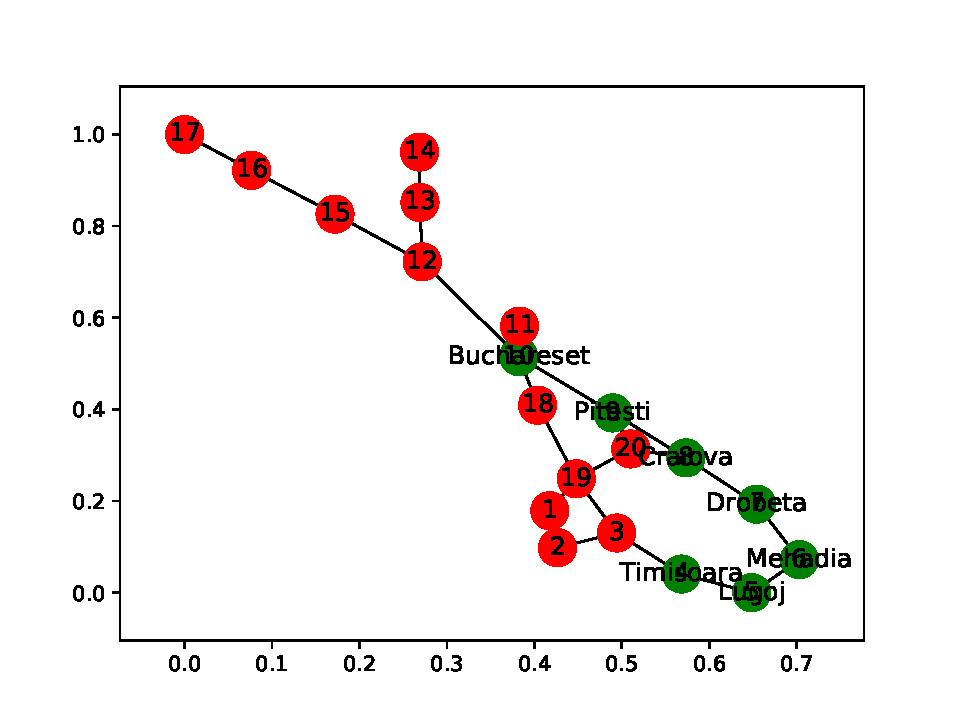
\includegraphics[width=.8\textwidth]{figures/graph}
	% \caption{$jkl$ }
	\label{gauss1}
\end{figure}

\section*{Exercise 5}
\begin{lstlisting}
Current node: Oradea
Best path: [1, 19, 20, 9, 10] Actual Path: [1, 19, 18, 10]
Current node: Zerind
Best path: [2, 3, 19, 20, 9, 10] Actual Path: [2, 3, 19, 18, 10]
Current node: Arad
Best path: [3, 19, 20, 9, 10] Actual Path: [3, 19, 18, 10]
Current node: Timisoara
Best path: [4, 3, 19, 20, 9, 10] Actual Path: [4, 5, 6, 7, 8, 9, 10]
Current node: Lugoj
Current node: Mehadia
Current node: Drobeta
Current node: Craiova
Current node: Pitesti
Current node: Buchareset
Current node: Giurgiu
Current node: Urziceni
Current node: Hirsova
Current node: Eforie
Current node: Vaslui
Current node: Iasi
Current node: Neamt
Current node: Fagaras
Current node: Sibiu
Best path: [19, 20, 9, 10] Actual Path: [19, 18, 10]
Current node: Rimnicu Vilcea
\end{lstlisting}

\newpage
\section{Appendix: Python Source Code}
Changed code to python3.
\lstinputlisting[language=Python]{uniform_cost_search.py}


\end{document}
